\let\negmedspace\undefined
\let\negthickspace\undefined
\documentclass[journal]{IEEEtran}
\usepackage[a5paper, margin=10mm, onecolumn]{geometry}
%\usepackage{lmodern} % Ensure lmodern is loaded for pdflatex
\usepackage{tfrupee} % Include tfrupee package

\setlength{\headheight}{1cm} % Set the height of the header box
\setlength{\headsep}{0mm}     % Set the distance between the header box and the top of the text

\usepackage{gvv-book}
\usepackage{gvv}
\usepackage{cite}
\usepackage{amsmath,amssymb,amsfonts,amsthm}
\usepackage{algorithmic}
\usepackage{graphicx}
\usepackage{textcomp}
\usepackage{xcolor}
\usepackage{txfonts}
\usepackage{listings}
\usepackage{enumitem}
\usepackage{mathtools}
\usepackage{gensymb}
\usepackage{comment}
\usepackage[breaklinks=true]{hyperref}
\usepackage{tkz-euclide} 
\usepackage{listings}
% \usepackage{gvv}                                        
\def\inputGnumericTable{}                                 
\usepackage[latin1]{inputenc}                                
\usepackage{color}                                            
\usepackage{array}                                            
\usepackage{longtable}                                       
\usepackage{calc}                                             
\usepackage{multirow}                                         
\usepackage{hhline}                                           
\usepackage{ifthen}                                           
\usepackage{lscape}
\begin{document}

\bibliographystyle{IEEEtran}
\vspace{3cm}

\title{12.9.6.14}
\author{EE24BTECH11019 - Dwarak A}
% \maketitle
% \newpage
% \bigskip
{\let\newpage\relax\maketitle}

\renewcommand{\thefigure}{\theenumi}
\renewcommand{\thetable}{\theenumi}
\setlength{\intextsep}{10pt} % Space between text and floats


\numberwithin{equation}{enumi}
\numberwithin{figure}{enumi}
\renewcommand{\thetable}{\theenumi}

\textbf{Question:}

Find the particular solution of the differential equation
\begin{align}
    \brak{1+x^2}\frac{dy}{dx}+2xy=\frac{1}{1+x^2}
\end{align}
for the inital condition $y = 0$, when $x = 1$.

\solution

\medskip

\textbf{Theoretical Solution:}
\begin{align}
    \frac{dy}{dx}+\brak{\frac{2x}{1+x^2}}y &= \frac{1}{\brak{1+x^2}^2}
\end{align}

Integrating factor,
\begin{align}
    \mu(x) &= e^{\int\frac{2x}{1+x^2}}dx \\
    \mu(x) &= 1+x^2
\end{align}

General solution,
\begin{align}
    y\brak{1+x^2} &= \int\frac{1}{1+x^2}dx \\
    y &= \frac{\tan^{-1}x + c}{1+x^2}
    \label{eqn:gen_soln}
\end{align}
where c is the constant of integration.

Substituting initial conditions, $x=1$ and $y=0$ in \eqref{eqn:gen_soln},
\begin{align}
    0 &= \frac{\tan^{-1}1 + c}{1+1^2} \\
    0 &= \frac{\frac{\pi}{4} + c}{2} \\
    c &= -\frac{\pi}{4}
    \label{eqn:int_const}
\end{align}

Particular solution obtained by substituting \eqref{eqn:int_const} in \eqref{eqn:gen_soln},
\begin{align}
    y &= \frac{\tan^{-1}x - \frac{\pi}{4}}{1+x^2}
\end{align}

\medskip

\textbf{Algorithm (Forward Euler Method):}

Definition of derivative,
\begin{align}
    f^\prime(x) &\approx \lim_{h\to0}\frac{f(x+h)-f(x)}{h} \\
    f(x+h) &\approx f(x)+hf^\prime(x) \\
    \implies y_{n+1} &\approx y_{n} + h\frac{dy}{dx}\Big|_{x=x_{n}, y=y_{n}}
\end{align}

Difference equation,
\begin{align}
    y_{n+1} &\approx y_{n} + h\brak{-\frac{2x_{n}y_{n}}{1+x_{n}^2} + \frac{1}{\brak{1+x_{n}^2}^2}} \\
    x_{n+1} &= x_{n}+h
\end{align}

\begin{figure}[h]
    \centering
    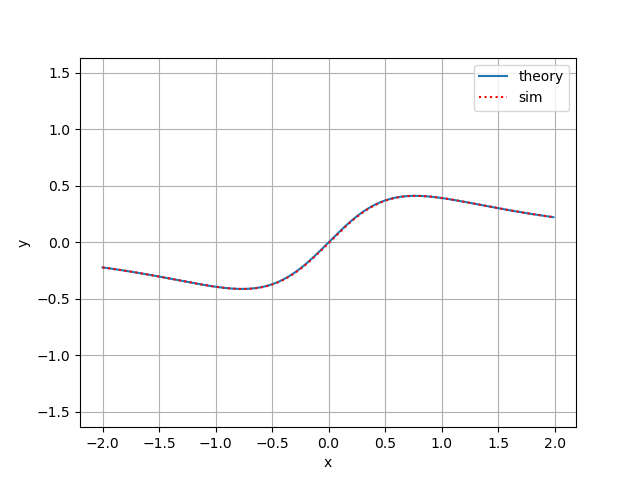
\includegraphics[width=\columnwidth]{figs/plot.png}
    \caption{Plot of the differential equation when $h=0.01$}
    \label{fig:Plot1}
    \end{figure}
\end{document}}
